\section{Evaluation}
\label{sec:evaluation}

In this Section, we present our experimental results.
First, we show the results about the randomness degree of the adopted pseudo-random number generator.
Then, we show the results about the performance recorded by the simulation of the target system.

% %
% EXPERIMENTAL ENVIRONMENT
% %
The experiments have been conducted on an Amazon EC2 c3.8xlarge instance, which is really indicated for high performance science and engineering applications\footnote{https://aws.amazon.com/ec2/instance-types/}.
The instance is equipped with 32 vCPU based on an Intel Xeon E5-2680 v2 (Ivy Bridge) processor, 30 GB of RAM and SSD with 900 IOPS.
It runs Debian 8.3 (Jessie), Python 3.5.2, and the Python-ported version of the official Leemis library for discrete-event simulation, indicated in \cite{leemis2006discrete}.
Our solution has been developed in Python, following the de-facto standard best-practices, stated in \cite{reitz2016,GooglePythonStyleguide}.

% %
% RANDOMNESS ANALYSIS
% %
\subsection{Randomness Analysis}
\label{sec:evaluation-randomness-analysis}
Let us now consider the results about the randomness degree of the adopted generator.
The randomness has been assessed by the following tests:

\begin{itemize}
	\item \textbf{Spectral Test:} this test is considered one of the most powerful tests to assess the quality of linear congruential generators \cite{knuth1981art}. It relies on the fact that the output of such generators form lines or hyperplanes when plotted on 2 or more dimensions. The less the distance between these lines or planes, the better the generator is. In fact, a smaller distance between lines or planes highlights a better uniform distribution.
	
	In Figure~\ref{fig:experimental-analysis-randomness-spectral-16807,fig:experimental-analysis-randomness-spectral-48271,fig:experimental-analysis-randomness-spectral-58012} we show the test results for generators $(16807,2^{31}-1)$, $(48271,2^{31}-1)$ and $(50812,2^{31}-1)$, respectively.
	
	The results show that our generator $(50812,2^{31}-1)$ is much better than $(16807, 2^{31}-1)$, which was a past de-facto standard, and it is really similar to $(48271,2^{31}-1)$, which is the current de-facto standard, according to \cite{leemis2006discrete}.
	
	\item \textbf{Test of Extremes:} this test relies on the fact that if $U=U_{0},...,U_{d-1}$ is an independent identically distributed sequence of $Uniform(0,1)$ random variables, then $\max(U)^{d}$ is also a $Uniform(0,1)$. The test leverages this property to measures, for every stream, how much the generated random values differ from the theoretical uniform distribution.
	
	Given a number of streams $s$ and a level of confidence $c=1-\alpha$, the more the total number of fails is close to the expected value, i.e. $s \cdot c$, the better the generator is.
	
	In Figure~\ref{fig:experimental-analysis-randomness-extremes-50812} we show the test results for the proposed generator $(508012,2^{31}-1, 256)$ with sample size $n=10000$, $k=1000$ bins, sequence size $d=5$ and $95\%$ level of confidence.
	%	
	The proposed generator shows critical values $v_{min}=913$ and $v_{max}=1088$ and 14 total fails (7 lower fails and 7 upper fails), that is not far from the theoretical accepted number of fails, i.e. $256*0.05=13$.
	The proposed generator successfully passed the test with a $94.531\%$ level of confidence.
	
	\item \textbf{Kolmogorov-Smirnov Analysis:} the test measures, at a given level of confidence, the biggest vertical distance between the theoretical cumulative distribution function and the empirical cumulative distribution function.
	The more the recorded distance $d$ is less than the critical value $d*$ for the considered level of confidence, the better the generator is.
	As the Kolmogorov-Smirnov analysis relies on pre-calculated randomness statistics, we have chosen to take into account the statistics obtained by the previous test.
	
	In Figure~\ref{fig:evaluation-randomness-kolmogorov-smirnov-50812} we show the test results for the proposed generator $(50812,2^{31}-1, 256)$ with a $95\%$ level of confidence.
	%
	The proposed generator successfully passed the test, as $d=0.041<0.081=d*$.
	
\end{itemize}

\begin{figure}
	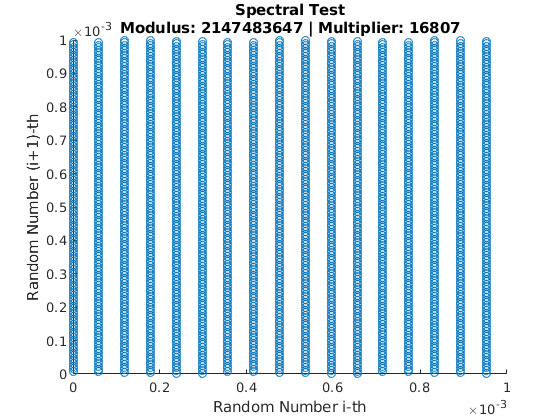
\includegraphics[width=\columnwidth]{fig/evaluation-randomness-spectral-16807}
	\caption{The Spectral Test to evaluate the randomness of the random number generator $(16807,2^{31}-1, 1)$ in the interval $(0, 10^{-3})$.}
	\label{fig:evaluation-randomness-spectral-16807}
\end{figure}

\begin{figure}
	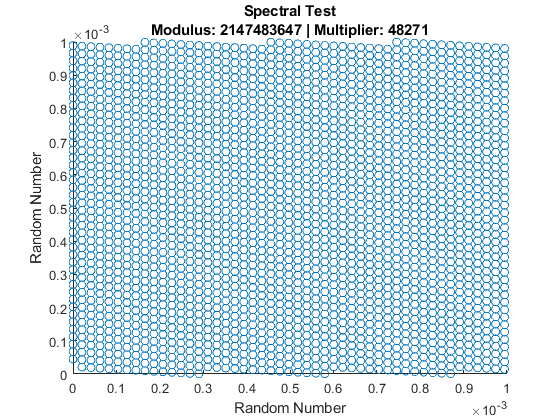
\includegraphics[width=\columnwidth]{fig/evaluation-randomness-spectral-48271}
	\caption{The Spectral Test to evaluate the randomness of the random number generator $(48271,2^{31}-1, 1)$ in the interval $(0, 10^{-3})$.}
	\label{fig:evaluation-randomness-spectral-48271}
\end{figure}

\begin{figure}
	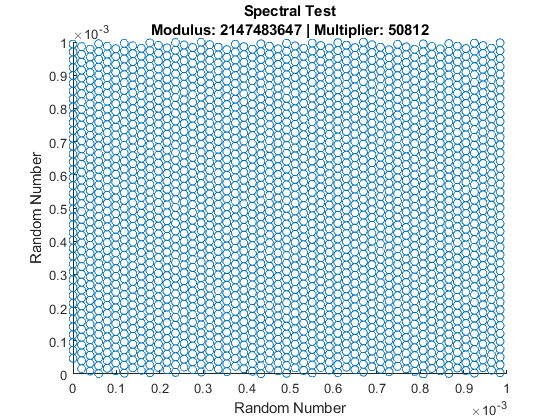
\includegraphics[width=\columnwidth]{fig/evaluation-randomness-spectral-50812}
	\caption{The Spectral Test to evaluate the randomness of the random number generator $(50812,2^{31}-1, 1)$ in the interval $(0, 10^{-3})$.}
	\label{fig:evaluation-randomness-spectral-50812}
\end{figure}

\begin{figure}
	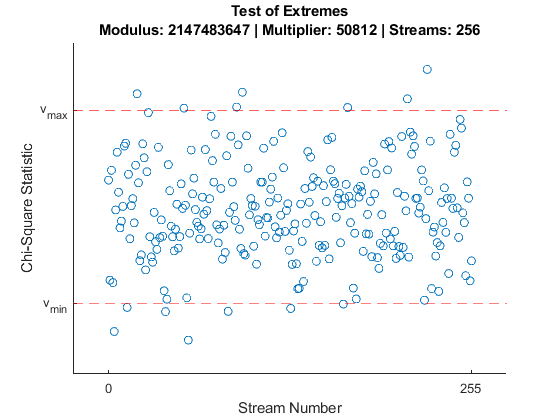
\includegraphics[width=\columnwidth]{fig/evaluation-randomness-extremes-50812}
	\caption{The Test of Extremes with $d=5$ to evaluate the randomness of the random number generator $(50812,2^{31}-1, 256)$.}
	\label{fig:evaluation-randomness-extremes-50812}
\end{figure}

\begin{figure}
	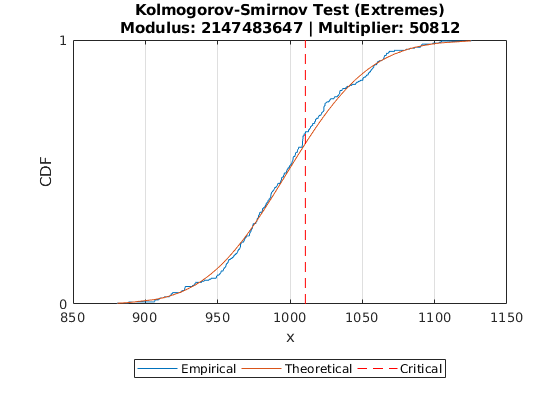
\includegraphics[width=\columnwidth]{fig/evaluation-randomness-kolmogorov-smirnov-50812}
	\caption{The Kolmogorov-Smirnov Analysis (leveraging the Test of Extremes with $d=5$) to evaluate the randomness of the random number generator $(50812,2^{31}-1, 256)$ with $0.95$ confidence level.}
	\label{fig:evaluation-randomness-kolmogorov-smirnov-50812}
\end{figure}


% %
% PERFORMANCE ANALYSIS
% %
\subsection{Performance Analysis}
Let us now consider the results about the performance recorded during the simulation of the target system.
In all the experiments we have considered the following parameters:

\begin{itemize}
	\item \textbf{arrivals:} exponential with rate $\lambda_{1}=6.00\;task/sec$ and $\lambda_{2}=6.25\;task/sec$.
	\item \textbf{services:} exponential with rate $\mu_{clt,1}=0.45\;task/sec$, $\mu_{clt,2}=0.27\;task/sec$, $\mu_{cld,1}=0.25\;task/sec$ and $\mu_{cld,2}=0.22\;task/sec$.
	\item \textbf{setup:} exponential with mean $E[T_{setup}]=0.8\;sec$.
\end{itemize}

\subsection{Transient Analysis}
\label{sec:evaluation-transient-analysis}
First, we conduct a \textit{transient analysis} to evaluate the stationary of the system and to estimate the duration of the transient period.
%
In fact, given a system that converges to stationary, the knowledge of the duration of the transient period is really important to conduct an effective performance evaluation. In particular, it allows the analyst to focus performance evaluation on a system in its stationary conditions.
%
In the transient analysis we focus on the following global metrics for the whole system: response time, throughout, mean population, ratio of switched tasks, response time for switched tasks. 
%
We assess the transient period of the aforementioned metrics because they are also the performance metrics that will be taken into account in the final performance evaluation, thus it is really important to study their stationary.

The following results have been produced by considering an ensemble of $5$ replications, where the $i+1$-th replication is initialized with the last seed of the $i$-th replication, so as to achieve the best decoupling between random sequences of different replications.

In Figure \ref{fig:evaluation-transient-analysis-response-time} we show the transient analysis of the global response time in the whole system.
%
In Figure \ref{fig:evaluation-transient-analysis-throughput} we show the transient analysis of the global throughput in the whole system.
%
In Figure \ref{fig:evaluation-transient-analysis-mean-population} we show the transient analysis of the global mean population in the whole system.
%
In Figure \ref{fig:evaluation-transient-analysis-switched-ratio} we show the transient analysis of the global switch ratio in the whole system.
%
In Figure \ref{fig:evaluation-transient-analysis-switched-response-time} we show the transient analysis of the response time for switched tasks in the whole system.

The results show that 
(i) the system is stationary,
(ii) the response time, the throughput, the mean population and the ratio of switched tasks loose their dependence on the starting conditions, whilst 
(iii) the response time for switched tasks maintains its dependence on starting conditions, regardless of the termination of the transient period.

As we could image, each metric exposes a distinct transient period, e.g. the ratio of switched tasks converges faster than the mean population. Thus, we consider $\tau*=8\cdot 10^{4}\;sec$ as the final instant of the transient period, as in $\tau*$ we are sure that all metrics loosed their dependence on starting conditions.

\begin{figure}
	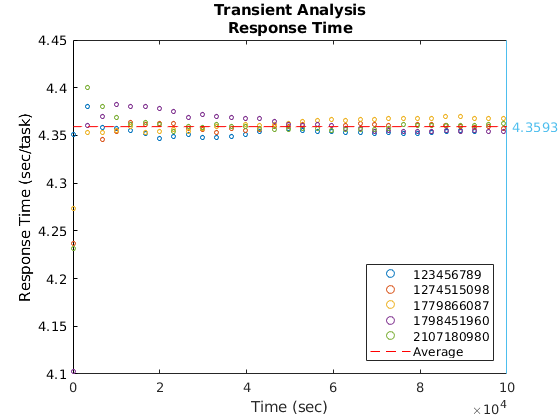
\includegraphics[width=\columnwidth]{fig/evaluation-transient-analysis-response-time}
	\caption{Transient analysis for global response time in the whole system.}
	\label{fig:evaluation-transient-analysis-response-time}
\end{figure}

\begin{figure}
	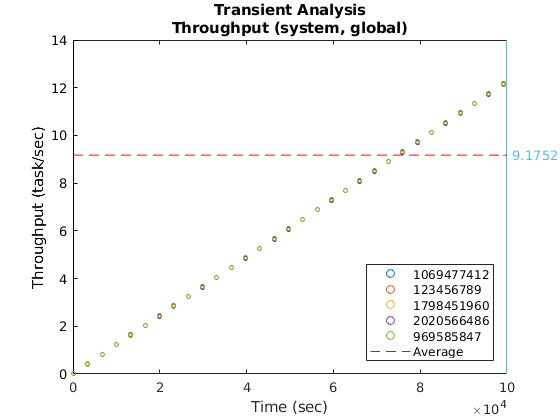
\includegraphics[width=\columnwidth]{fig/evaluation-transient-analysis-throughput}
	\caption{Transient analysis for global throughput in the whole system.}
	\label{fig:evaluation-transient-analysis-throughput}
\end{figure}

\begin{figure}
	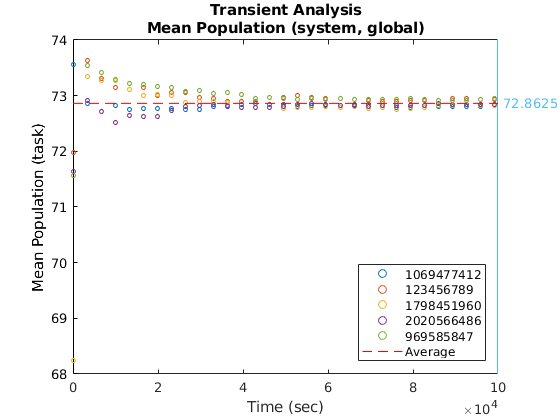
\includegraphics[width=\columnwidth]{fig/evaluation-transient-analysis-mean-population}
	\caption{Transient analysis for global mean population in the whole system.}
	\label{fig:evaluation-transient-analysis-mean-population}
\end{figure}

\begin{figure}
	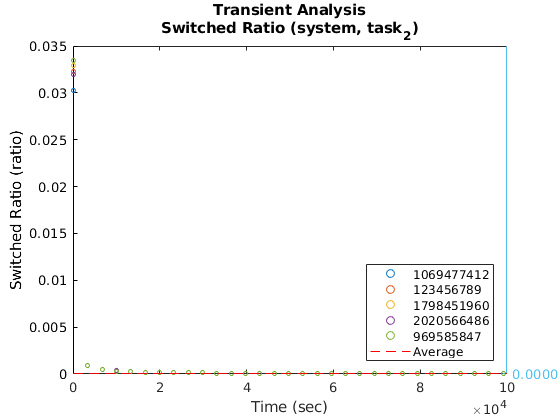
\includegraphics[width=\columnwidth]{fig/evaluation-transient-analysis-switched-ratio}
	\caption{Transient analysis for the ratio of switched tasks of type 2.}
	\label{fig:evaluation-transient-analysis-switched-ratio}
\end{figure}

\begin{figure}
	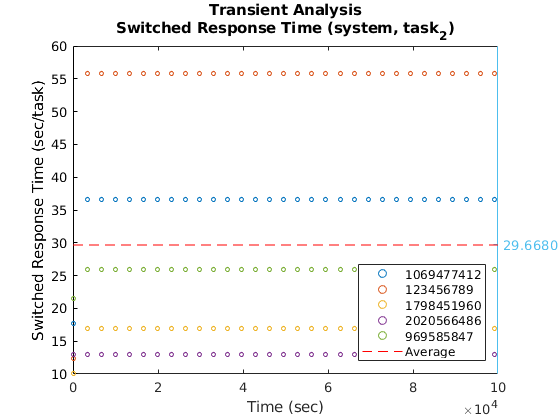
\includegraphics[width=\columnwidth]{fig/evaluation-transient-analysis-switched-response-time}
	\caption{Transient analysis for response time for switched tasks of type 2.}
	\label{fig:evaluation-transient-analysis-switched-response-time}
\end{figure}


\subsection{Performance Evaluation}
Let us now focus on the \textit{performance evaluation}, taking into account the following metrics:

\begin{enumerate}
	\item response time both global and per-class, both for the system as a whole and for each subsystem;
	\item throughput both global and per-class, both for the system as a whole and for each subsystem;
	\item mean population both global and per-class, both for the system as a whole and for each subsystem;
	\item ratio of switched tasks of type 2;
	\item response time for switched tasks of type 2.
\end{enumerate}

\begin{figure}
	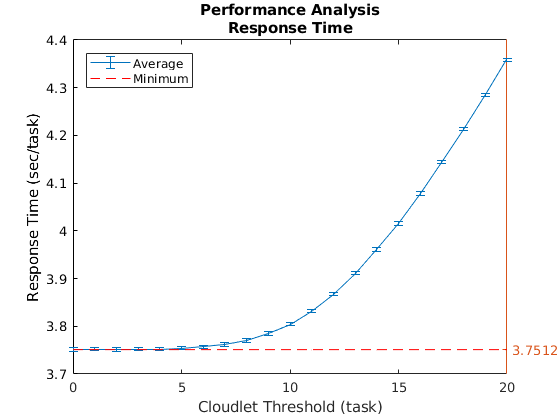
\includegraphics[width=\columnwidth]{fig/evaluation-performance-analysis-response-time}
	\caption{Performance analysis of response time as a function of the threshold $S$ with level of confidence $95\%$. The threshold that minimizes the response time is $S*=2$ with mean value $E[R]\approx3.7512 \; sec$.}
	\label{fig:evaluation-performance-analysis-response-time}
\end{figure}

\begin{figure}
	\begin{center}
	\begin{tabular}{|c||c|c|}
		\hline
		$\mathbf{S}$ & $\mathbf{\mu(R)\pm\delta_{0.05}}$ & $\mathbf{\sigma(R)}$\\
		\hline
		$0$  & $3.75149\pm 0.00342$ & $0.01346$ \\
		$1$  & $3.75172\pm 0.00335$ & $0.01322$ \\
		$\mathbf{2}$  & $\mathbf{3.75120\pm 0.00338}$ & $\mathbf{0.01330}$ \\
		$3$  & $3.75198\pm 0.00334$ & $0.01315$ \\
		$4$  & $3.75200\pm 0.00328$ & $0.01292$ \\
		$5$  & $3.75430\pm 0.00324$ & $0.01275$ \\
		$10$ & $3.80394\pm 0.00330$ & $0.01299$ \\
		$15$ & $4.01623\pm 0.00406$ & $0.01599$ \\
		$20$ & $4.35885\pm 0.00342$ & $0.01349$ \\
		\hline
	\end{tabular}
	\end{center}
	\caption{Performance analysis of the response time as a function of the threshold $S$ with level of confidence $95\%$.}
	\label{tbl:evaluation-performance-analysis-response-time}
\end{figure}

\begin{figure}
	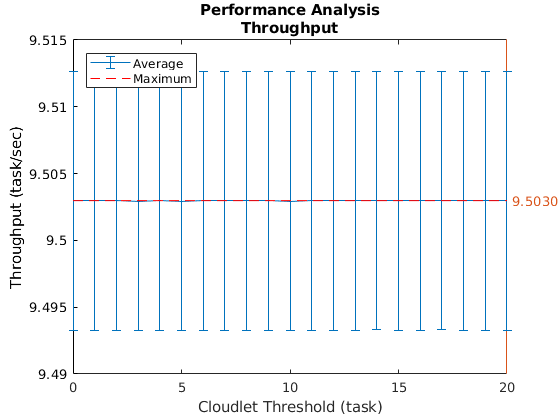
\includegraphics[width=\columnwidth]{fig/evaluation-performance-analysis-throughput}
	\caption{Performance analysis of the throughput as a function of the threshold $S$  with level of confidence $95\%$. The throughput is clearly threshold insensitive, with a constant mean value $E[X]\approx9.5030 \; task/sec$. The threshold $S*=2$ is a good choice}
	\label{fig:evaluation-performance-analysis-throughput}
\end{figure}

\begin{figure}
	\begin{center}
		\begin{tabular}{|c||c|c|}
			\hline
			$\mathbf{S}$ & $\mathbf{\mu(X)\pm\delta_{0.05}}$ & $\mathbf{\sigma(X)}$\\
			\hline
			$0$  & $9.50296\pm 0.00969$ & $0.03818 $ \\
			$1$  & $9.50295\pm 0.00969$ & $0.03818$ \\
			$\mathbf{2}$  & $\mathbf{9.50296\pm 0.00969}$ & $\mathbf{0.03816}$ \\
			$3$  & $9.50294\pm 0.00967$ & $0.03808$ \\
			$4$  & $9.50296\pm 0.00969$ & $0.03816$ \\
			$5$  & $9.50294\pm 0.00969$ & $0.03818$ \\
			$10$ & $9.50295\pm 0.00969$ & $0.03818$ \\
			$15$ & $9.50295\pm 0.00968$ & $0.03813$ \\
			$20$ & $9.50296\pm 0.00970$ & $0.03821$ \\
			\hline
		\end{tabular}
	\end{center}
	\caption{Performance analysis of the throughput as a function of the threshold $S$ with level of confidence $95\%$.}
	\label{tbl:evaluation-performance-analysis-throughput}
\end{figure}

\begin{figure}
	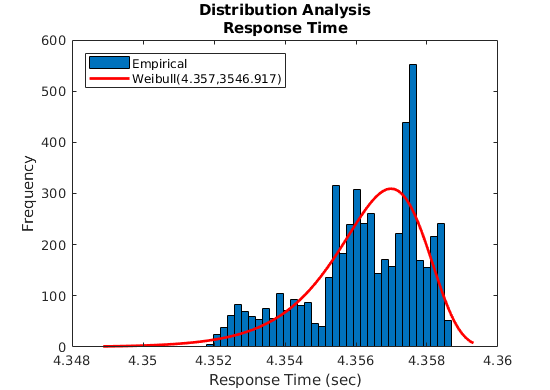
\includegraphics[width=\columnwidth]{fig/evaluation-distribution-analysis-response-time}
	\caption{Distribution analysis for response time with threshold $S=20$. The binnign rule is Freedman-Diaconis Rule. The best fitting is the Weibull with parameters $A\approx4.357$ and $B\approx3546.917$.}
	\label{fig:evaluation-distribution-analysis-response-time}
\end{figure}

%%
% DISTRIBUTION ANALYSIS
%%
\subsection{Distribution Analysis}
\label{sec:evaluation-distribution-analysis}